% !TeX root = ../note.tex
\subsection{Обзор существующих аналогов}\label{sec:analysis:analogues}

В данном разделе рассмотрим существующие аналоги, а именно системы, обладающие механизмами для создания ордеров, совершения сделок и другим соответствующим функционалом.

% \subsubsection{} Exchange-core\label{sec:analysis:analogue_1}
\textbf{Exchange-core}

Exchange-core~\cite{analogue_1} позиционируется как высокоскоростная система матчинга ордеров написанная на Java и использующая такие технологии как:
\begin{itemize}
    \item LMAX Disruptor — высокопроизводительная межпоточная библиотека сообщений — библиотека, использующаяся для передачи ордеров и сделок между потоками, для синхронизации процессов получения ордеров и записи сделок в БД.
    \item Eclipse Collections — фреймворк коллекций для Java, превосходящих по скорости встроенные коллекции JDK (Java Development Kit);
    \item Real Logic Agrona — набор высокопроизводительных структур данных и утилитарных методов для Java;
    \item OpenHFT's Chronicle-Queue — быстрая очередь сообщений, с возможностью хранения данных на жёстком диске.
    \item LZ4 Java — библиотека для компрессии данных в формате lz4, написанная на Java, обладающая высокой скоростью сканирования данных и отличающаяся высоким коэффициентом компрессии данных.
\end{itemize}

\begin{figure}[ht]
    \centering
	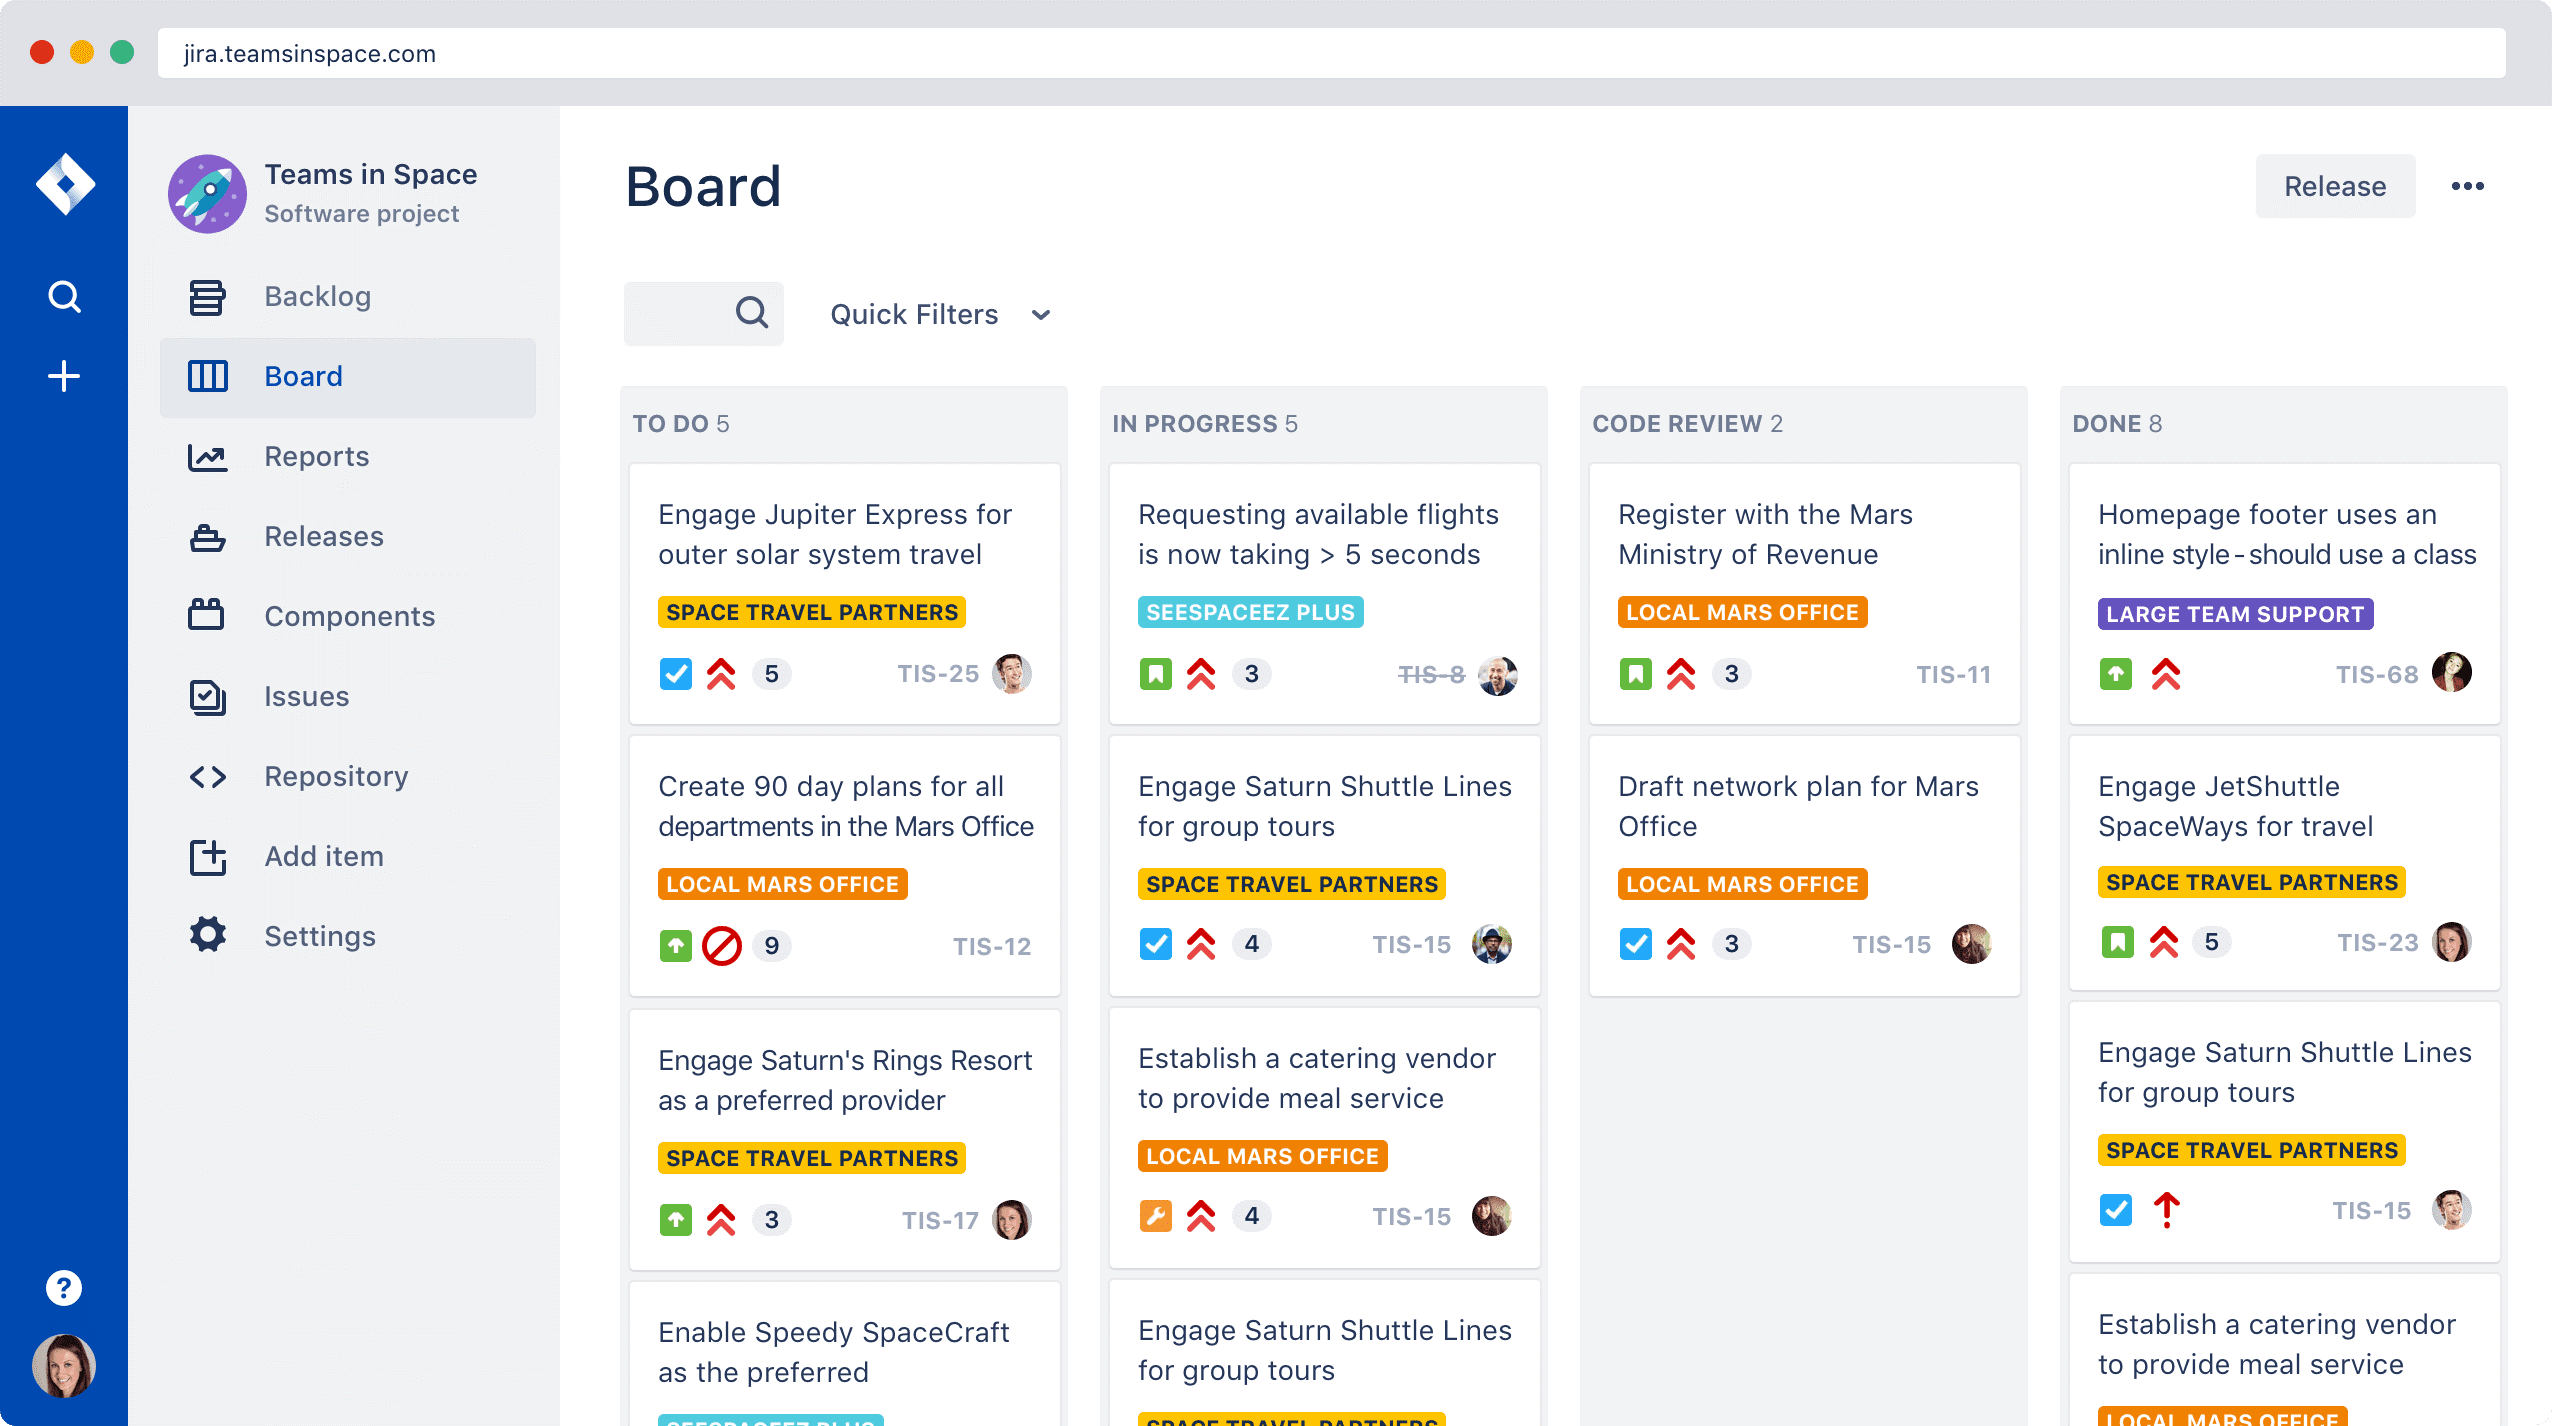
\includegraphics[width=\textwidth]{analogue_1.png}
	\caption{Бенчмарки для exchange-core}\label{fig:analysis:analogue_1:picture}
\end{figure}

Из плюсов данного проекта можно отметить:
\begin{itemize}
    \item оптимизирована для HFT (высокочастотной торговли);
    \item состояние биржевого стакана и сбор данных ведутся в оперативной памяти;
    \item наличие различных видов тестирования системы — юнит-тесты, интеграционные тесты, стресс-тесты и тесты на целостность данных;
    \item отсутствие математики с ''плавающей точкой`` для повышения точности вычислений;
    \item наличие режимов для оценки рисков.
\end{itemize}

К минусам данного ПО можно отнести:
\begin{itemize}
    \item отсутствие хранения какой-либо пользовательской информации, в силу чего невозможно организовать проверки на валидность совершения операций и наличие баланса для проведения операций. Поэтому данные вещи необходимо организовывать силами третьей стороны;
    \item проект написан на Java, поэтому предполагает наличие Java Virtual Machine, что является прослойкой между ПО и системой, на которой оно запущено. JVM хорошо использовать для обеспечения кроссплатформенности проекта, но само его наличие негативно влияет на скорость выполнения операции в ПС.
    \item отсутствие логирования происходящего в движке;
    \item отсутствие механизма ''чистого`` перезапуска системы.
\end{itemize}

% \subsubsection{} Gitbitex-spot
\textbf{Gitbitex-spot}

Gitbitex-spot — ПС для криптовалютной биржи, написанный на Golang с использованием Kafka, Redis и MySQL СУБД~\cite{analogue_2}.

\begin{figure}[ht]
    \centering
	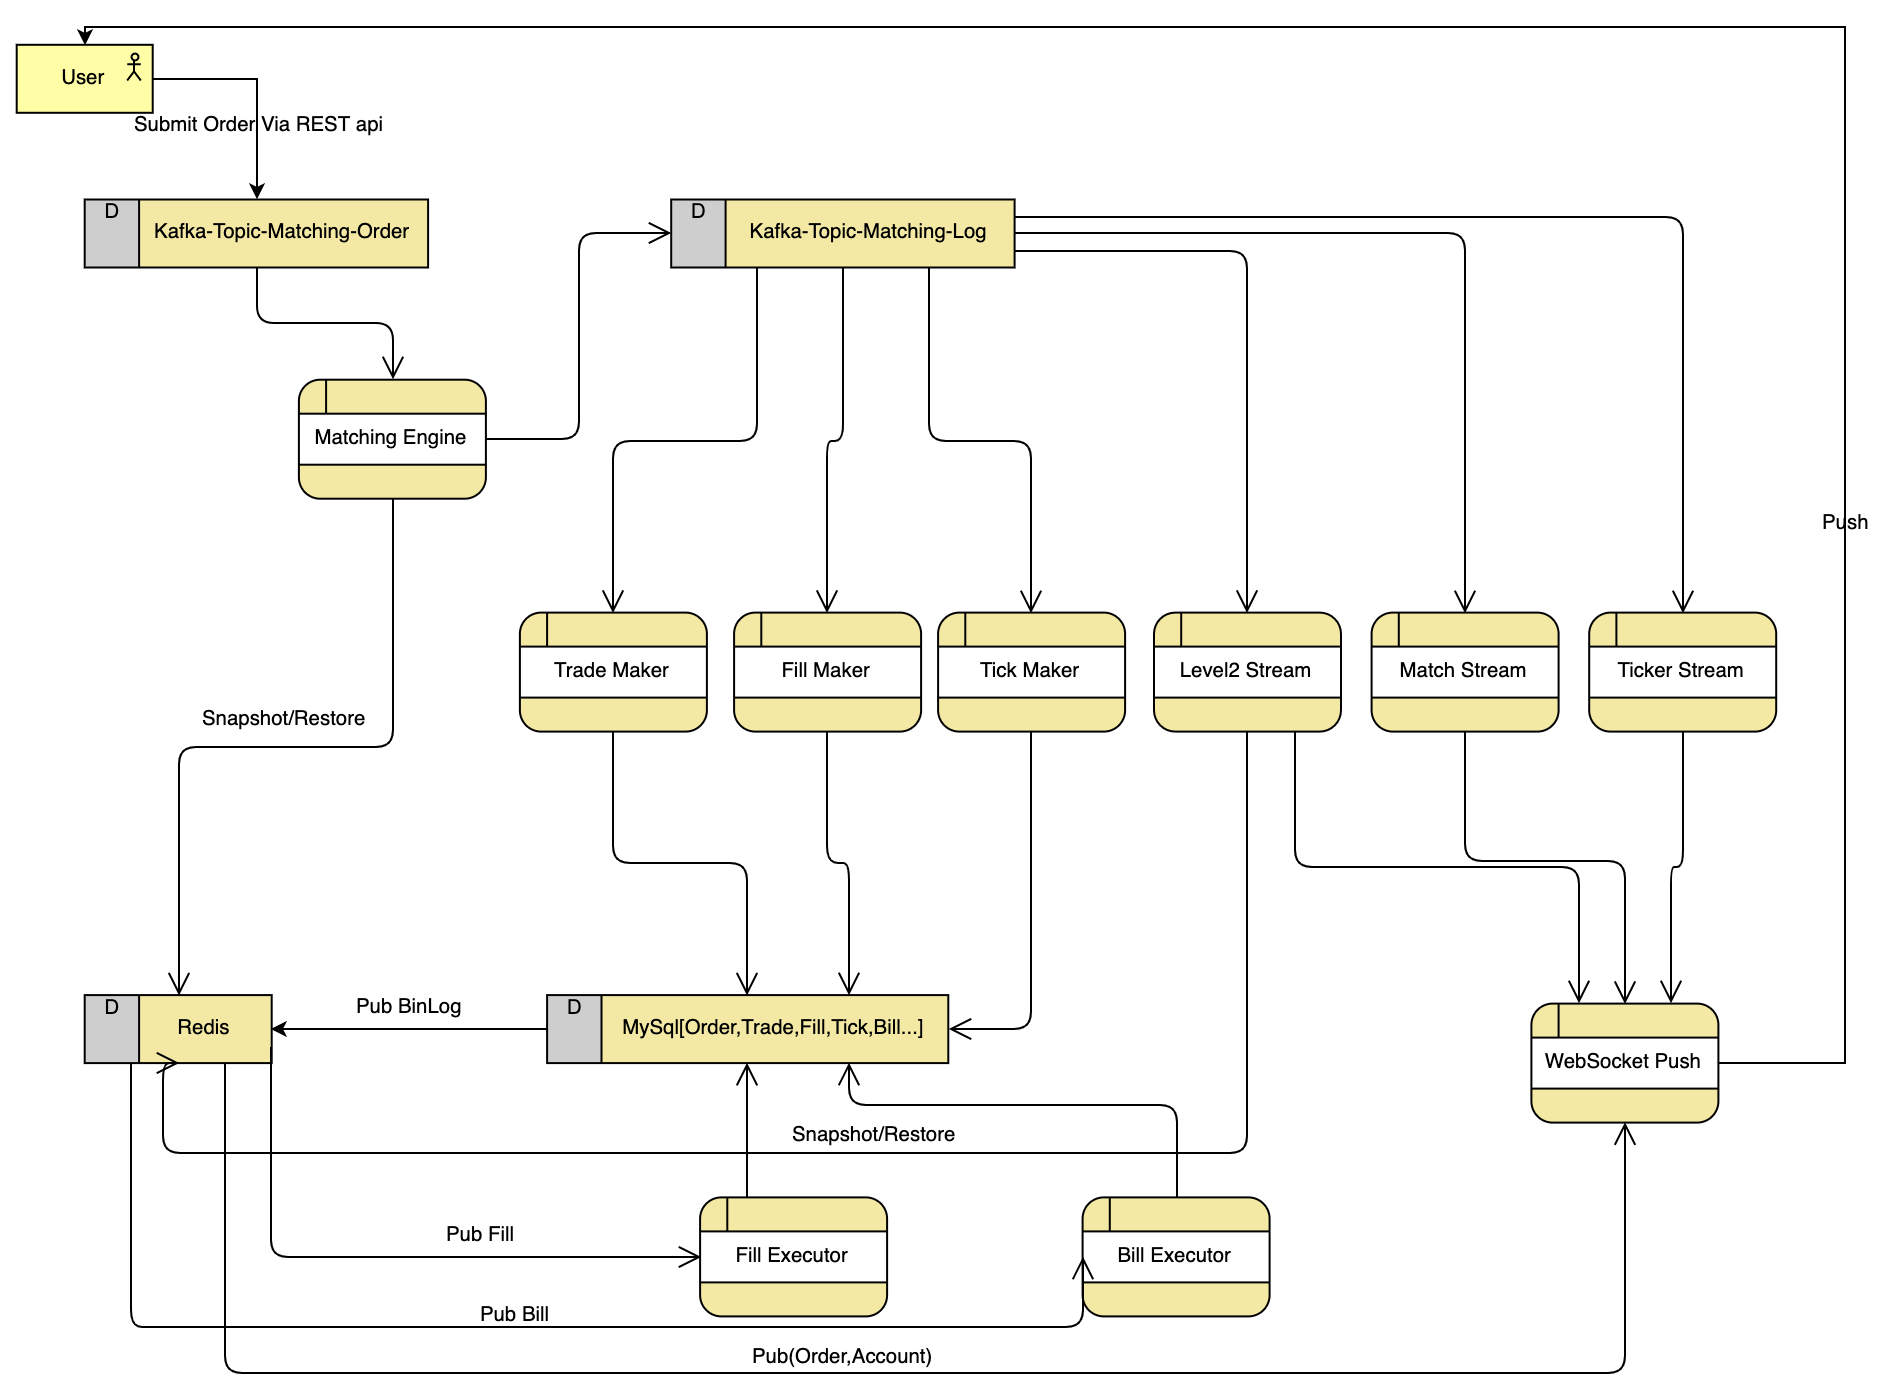
\includegraphics[width=\textwidth]{analogue_2.png}
	\caption{Архитектура gitbitex-spot}\label{fig:analysis:analogue_2:picture}
\end{figure}

В данном проекте можно отметить как плюсы следующее:
\begin{itemize}
    \item проект написан на Golang, который является относительно новым и быстрым языком (по сравнению с Java, который используется в Exchange-core), а также предоставляет удобные встроенные инструменты для работы с несколькими потоками;
    \item использование СУБД MySQL с опцией BINLOG[ROW format], которая позволяет более эффективно хранить и читать данные, специфичные для данной системы.
    \item наличие простейшего front-end, который храниться отдельно от системы, что говорит о её независимости от пользовательского интерфейса.
\end{itemize}

К минусам данного ПО можно отнести:
\begin{itemize}
    \item отсутствие документации API для подключения и использования системы;
    \item отсутствие замеров производительности системы;
    \item отказоустойчивость для всей системы не предусмотрена, существует только на уровне отдельных технологий;
    \item согласно goreportcard, в проекте существует множество неисправленных предупреждений, которые потенциально могут привести к ошибкам в расчётах или безопасности.
\end{itemize}

% \subsubsection{} CppTrader
\textbf{CppTrader}

CppTrader — набор компонентов для построения высокопроизводительной торговой платформы~\cite{analogue_3}. Проект не является полноценной рабочей системой, но содержит в себе множество важных компонентов, необходимых для построения торговой платформы, поэтому его можно сравнивать с другими системами с помощью его компонентов.

\begin{figure}[ht]
\centering
    \centering
    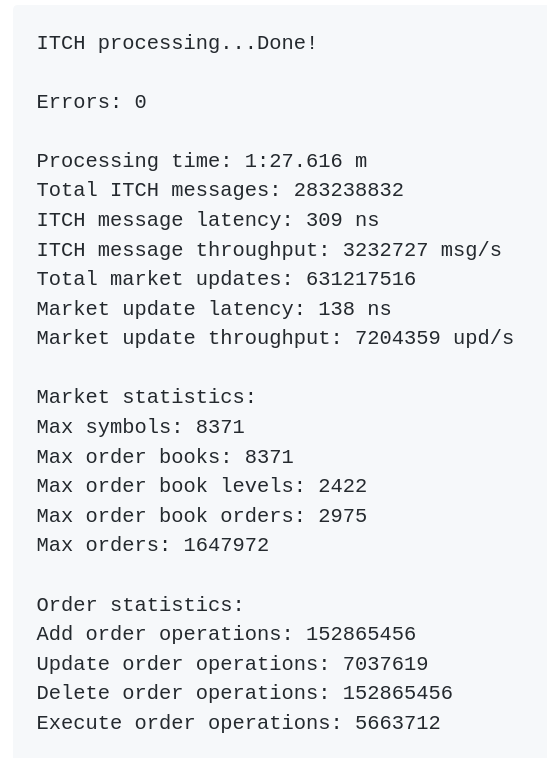
\includegraphics[width=0.5\textwidth]{analogue_3_1.png}
    \caption{Market manager бенчмарк}\label{fig:analysis:analogue_3:picture_1}
\end{figure}
\begin{figure}[ht]
    \centering
    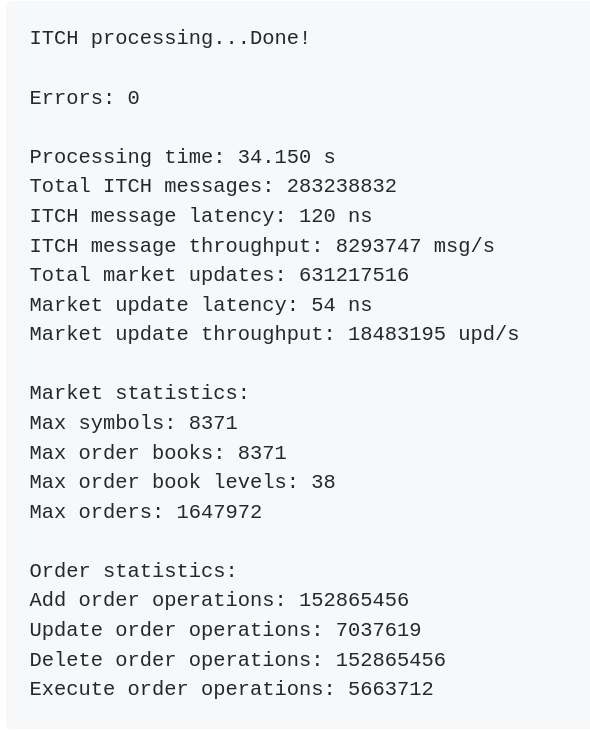
\includegraphics[width=0.5\textwidth]{analogue_3_2.png}
    \caption{Оптимизированный market manager бенчмарк}\label{fig:analysis:analogue_3:picture_2}
\end{figure}

Из сильных сторон проекта можно выделить:
\begin{itemize}
    \item реализация ITCH (не имеет расшифровки) интерфейса для взаимодействия с NASDAQ;\@
    \item высокая скорость работы матчинга ордеров;
    \item наличие средств для управления ''биржевым стаканом``.
    \item наличие документации, которая генерируется через Doxygen.
\end{itemize}

Слабые стороны проекта выделять не будем, так как это лишь частично аналогичная разработка, и её минусы будут лишь архитектурными решениями, изначально заложенными в данный проект.
